\section{Measuring Goodharting}\label{appendix:measuring_goodharting}

While Goodhart’s law is qualitatively well-described, a quantitative measure is needed to systematically analyse it. We propose a number of different metrics to do that. Below, implicitly assuming that all rewards are normalised (as in the~\Cref{sec:preliminaries}), we denote by $f: [0, 1] \to [0, 1]$ the true reward obtained by a policy trained on a \emph{proxy reward}, as a function of optimisation pressure $\lambda$, similarly by $f_0$ the true reward obtained by a policy trained on the \emph{true reward}, and $\lambda^\star = \arg\max_{\lambda \in [0, 1]} f(\lambda)$.

\begin{itemize}
    \item \textbf{Normalised drop height:} 
    \[
        \text{NDH}(f) = f(1) - f(\lambda^\star)
    \]
    \item \textbf{Simple integration:} 
    \[
        \text{SI}(f) = \left( \int_{0}^{\lambda^\star} f(\lambda) d\lambda \right) \left( \int_{\lambda^\star}^1 f(\lambda) d\lambda \right)
    \]
    \item \textbf{Weighted correlation-anticorrelation:} 
    \[
    \text{CACW}(f) = -\max(\rho_0, 0) \max(\rho_1, 0) \sqrt{\lambda^\star (1- \lambda^\star)}
    \]
    where $\rho^i = \rho(f(I_i), I_i)$ are the Pearson correlation coefficients for $I_0 \sim Unif[0, \lambda^\star]$, $I_1 \sim Unif[\lambda^\star, 1]$.
    \item \textbf{Regression angle:} 
    \[
        \text{LR}(f) = -\beta_0^+ \beta_1^+
    \] where $\beta_0, \beta_1$ are the angles of the linear regression of $f$ on $[0, \lambda^\star]$ and $[\lambda^\star, 1]$ respectively.
    \item \textbf{Relative weighted integration:} \[
        \text{RWI}(f) = \left((1 - \lambda^\star) \int_{0}^{\lambda^\star} |f(\lambda) - f_0(\lambda)| d\lambda \right) \left(\frac{1}{1 - \lambda^\star} \int_{\lambda^\star}^1 |f(\lambda) - f_0(\lambda)| d\lambda \right) 
        \]
\end{itemize}

The metrics were independently designed to capture the intuition of a \emph{sudden drop in reward with an increased optimisation pressure}. We then generated a dataset of 40000 varied environments: 
\begin{itemize}
\item \emph{Gridworld}, \textbf{Terminal} reward, with $|S| \sim Poiss(100)$, N=1000
\item \emph{Cliff}, \textbf{Cliff} reward, with $|S| \sim Poiss(100)$, N=500
\item \emph{RandomMDP}, \textbf{Terminal} reward, $|S| \sim Poiss(100)$, $|A| \sim Poiss(6)$, N=500
\item \emph{RandomMDP}, \textbf{Terminal} reward, $|S| \sim Unif(16, 64), |A| \sim Unif(2, 16)$, N=500
\item \emph{RandomMDP}, \textbf{Uniform} reward, $|S| \sim Unif(16, 64), |A| \sim Unif(2, 16)$, N=500
\item \emph{CyclicMDP}, \textbf{Terminal} reward, $\text{depth} \sim Poiss(3)$, N=1000
\end{itemize}

We have manually verified that all metrics seem to activate strongly on graphs that we would intuitively assign a high degree of Goodharting. In~\Cref{fig:highest-scores}, we show, for each metric, the top three training curves from the dataset that each metric assigns the highest score.

We find that all of the metrics are highly correlated - see~\Cref{table:goodhart-metric-correlations}. Because of this, we believe that it is meaningful to talk about a quantitative Goodharting score. Since normalised drop height is the simplest metric, we use it as the proxy for Goodharting in the rest of the paper.

\begin{figure}
    \centering
    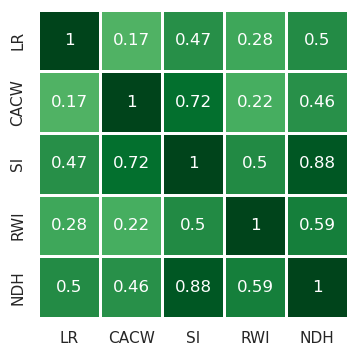
\includegraphics[width=0.3\textwidth]{metrics/metrics_correlations.png}
    \caption{Correlations between different Goodharting metrics, computed over examples where the drop occurs for $\lambda > 0.3$, to avoid selecting adversarial examples.}
    \label{table:goodhart-metric-correlations}
\end{figure}


\begin{figure}[htbp]
    \centering
    \begin{subfigure}[tb]{0.6\textwidth}
            \centering
            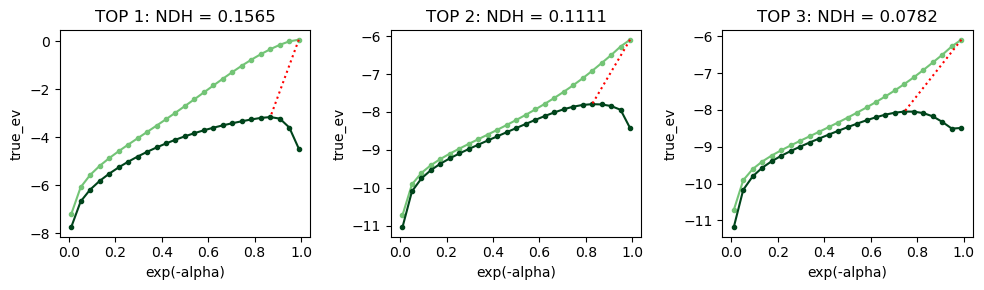
\includegraphics[width=\textwidth]{metrics/topmetric_ndh.png}
            \caption{Top 3 curves according to NDH metric.}
            \label{fig:topmetric-ndh}
    \end{subfigure}
    \hfill
    \begin{subfigure}[tb]{0.6\textwidth}
            \centering
            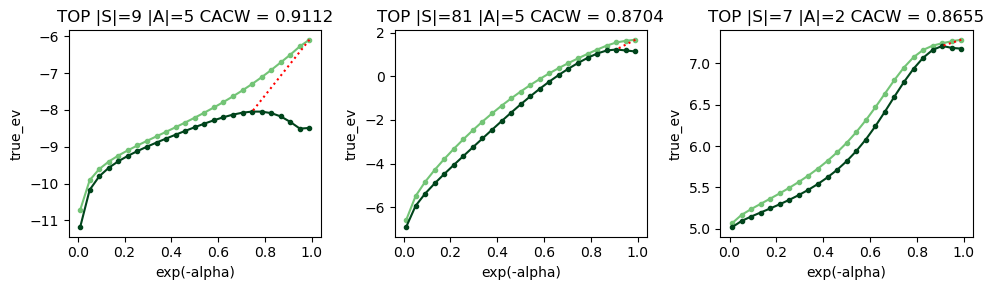
\includegraphics[width=\textwidth]{metrics/topmetric_cacw.png}
            \caption{Top 3 curves according to CACW metric.}
            \label{fig:topmetric-cacw}
    \end{subfigure}
    \hfill
    \begin{subfigure}[tb]{0.6\textwidth}
            \centering
            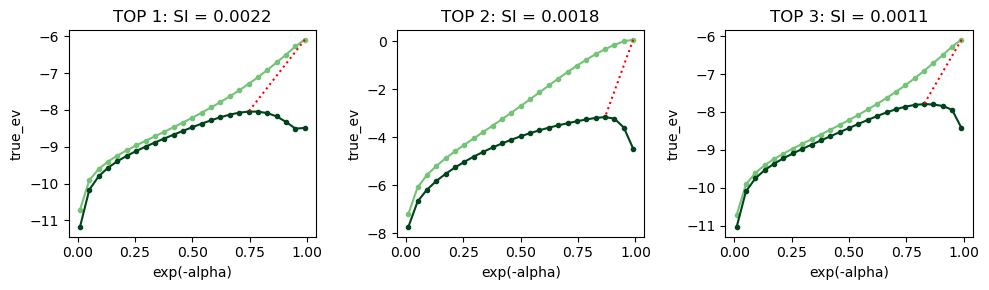
\includegraphics[width=\textwidth]{metrics/topmetric_si.png}
            \caption{Top 3 curves according to SI metric.}
            \label{fig:topmetric-si}
    \end{subfigure}
    \hfill
    \begin{subfigure}[tb]{0.6\textwidth}
            \centering
            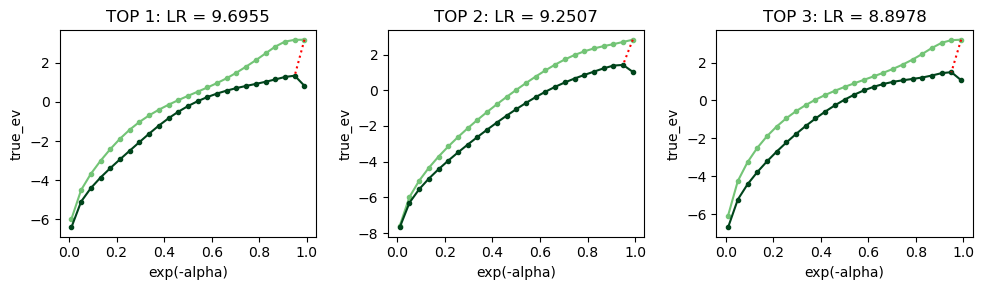
\includegraphics[width=\textwidth]{metrics/topmetric_lr.png}
            \caption{Top 3 curves according to LR metric.}
            \label{fig:topmetric-lr}
    \end{subfigure}
    \hfill
    \begin{subfigure}[tb]{0.6\textwidth}
            \centering
            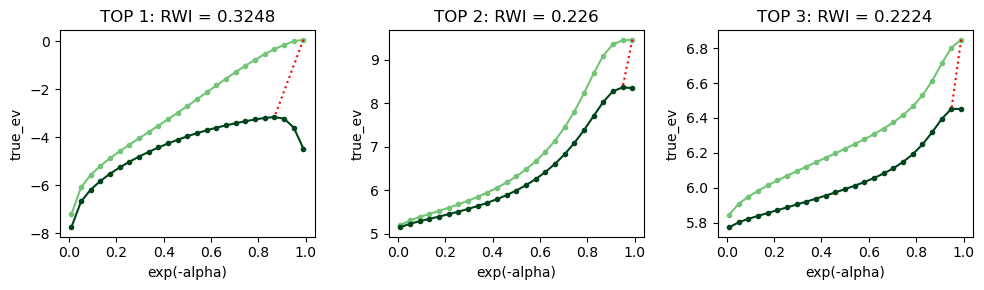
\includegraphics[width=\textwidth]{metrics/topmetric_rwi.png}
            \caption{Top 3 curves according to RWI metric.}
            \label{fig:topmetric-rwi}
    \end{subfigure}
    \caption{Examples of training curves that obtain high Goodharting scores according to each metric.\label{fig:highest-scores}}
\end{figure}

